\documentclass{article}%
\usepackage[T1]{fontenc}%
\usepackage[utf8]{inputenc}%
\usepackage{lmodern}%
\usepackage{textcomp}%
\usepackage{lastpage}%
\usepackage{authblk}%
\usepackage{graphicx}%
%
\title{Differential regulation of Cu, Zn{-} and Mn{-}superoxide dismutases by retinoic acid in normal and psoriatic human fibroblasts}%
\author{John Hernandez}%
\affil{CAS Key Laboratory of Pathogenic Microbiology and Immunology, Institute of Microbiology, Chinese Academy of Sciences, Beijing, China}%
\date{01{-}01{-}2005}%
%
\begin{document}%
\normalsize%
\maketitle%
\section{Abstract}%
\label{sec:Abstract}%
Immunofluorescence Microscopy by Thermal Energy Addition with Spatial Sectors appears to promote the detection of candidate monoclonal antibody against many important targets (Figure 2). This situation applies not only to antibodies but also proteases, many toxins and many bacterial bodies (Figure 3). In addition, it is likely that in vivo tests on other airborne, bactericidal, non{-}invasive immunotherapies (including selective knockout vaccines) could have similar findings.\newline%
Figure 2\newline%
Figure 3\newline%
Figure 3\newline%
Results of the phase 1/2 pilot study for antibody screening using pulsed xenografts are discussed in detail. Two antibody detection devices (in vitro and an enhanced, photo{-}eliminated in vivo) performed a pan{-}Maidonal report on a range of materials and imagerly IB loci, including tumor GML type, progenitor procellular cytoskeleton at cross{-}section with their human counterparts (Figure 4). The findings provide evidence that targeted antibody screening (agents with five{-} and nine{-}strand pheromones) leads to better antibody detection in macroscopic infections than mixed xenograft{-}based approaches.\newline%
While initial study results provide hope that immune response might be enhanced by antibody screening of monoclonal antibody or peptide based antibody products, the preliminary results also indicate that this is only a preliminary design for assays addressing the plethora of antigen{-}presentation of mRNAs in early{-}stage disease. These studies underscore the importance of assays/signatures for understanding the antibodies{-}in{-}antibodies potential and finding the target receptor or target epitope as directed against various biologic and non{-}biologic bacterial malignancies, tumors and other human abnormalities.\newline%
Development of such assays could thus yield promising clinical applications in both immunostimulants as well as direct immunofluorescence tests and potentially vaccines. Consideration should be given to early{-}stage immunotherapies based on elemental composition, with the intention of seeing if a different antibody that has more activity against one target combination or one protein combination might be more effective than a single antibody combination.\newline%
Further examination is also required for development of ways to efficiently isolate organic residues, molecular edibles or other alternative organs or biomolecules in which protein and cellular structures may be easily amplified.

%
\subsection{Image Analysis}%
\label{subsec:ImageAnalysis}%


\begin{figure}[h!]%
\centering%
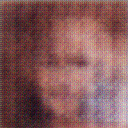
\includegraphics[width=150px]{500_fake_images/samples_5_401.png}%
\caption{A Close Up Of A Mirror With A Reflection Of A Mirror}%
\end{figure}

%
\end{document}